%-----------------------------------LICENSE------------------------------------%
%   This file is part of Mathematics-and-Physics.                              %
%                                                                              %
%   Mathematics-and-Physics is free software: you can redistribute it and/or   %
%   modify it under the terms of the GNU General Public License as             %
%   published by the Free Software Foundation, either version 3 of the         %
%   License, or (at your option) any later version.                            %
%                                                                              %
%   Mathematics-and-Physics is distributed in the hope that it will be useful, %
%   but WITHOUT ANY WARRANTY; without even the implied warranty of             %
%   MERCHANTABILITY or FITNESS FOR A PARTICULAR PURPOSE.  See the              %
%   GNU General Public License for more details.                               %
%                                                                              %
%   You should have received a copy of the GNU General Public License along    %
%   with Mathematics-and-Physics.  If not, see <https://www.gnu.org/licenses/>.%
%------------------------------------------------------------------------------%
%       Author: Ryan Maguire                                                   %
%       Date:   2024/03/07                                                     %
%------------------------------------------------------------------------------%
\documentclass{article}
\usepackage{amssymb}
\usepackage{amsmath}
\usepackage{amsthm}
\usepackage{graphicx}
\usepackage{hyperref}
\hypersetup{colorlinks = true, linkcolor = blue}
\setlength{\parindent}{0em}
\setlength{\parskip}{0em}
\graphicspath{{../images/}}
\theoremstyle{plain}
\newtheorem{theorem}{Theorem}

% Title page information.
\title{Tait Graphs for Virtual Knots}
\author{Ryan Maguire}
\date{\today}
\begin{document}
    \maketitle
    \tableofcontents
    \begin{abstract}
        A generalization of the Tait graph for classical knots is presented
        for virtual knots.
    \end{abstract}
    \section{Gauss Codes}
        \begin{figure}
            \centering
            \resizebox{0.5\textwidth}{!}{%
                \includegraphics{%
                    trefoil_knot_oriented_with_gauss_code.pdf
                }
            }
            \caption{Gauss Code for the Right-Handed Trefoil}
            \label{fig:right_handed_trefoil_gauss_code}
        \end{figure}
        Given an \textit{oriented} knot diagram $K$ with $N$ crossings, we
        label the crossings $0$ to $N-1$. Any ordering will suffice, but
        usually one picks a point and then travels along the knot, following
        the orientation, and labels the crossings in increasing order as they
        pass. Now pick a starting point and follow along the knot. As you
        come upon a crossing write down its number and whether you are on the
        over strand or the under strand. Do this until you return to your
        starting point. Each crossing will occur twice in your list, once as an
        over crossing and once as an under crossing, so at the end you will
        have a sequence with $2N$ entries. This is called the
        \textbf{unsigned Gauss code} of the knot. It is dependent on the
        knot diagram, your choice of labeling, the orientation given, and your
        choice in starting point. Consider
        Fig.~\ref{fig:right_handed_trefoil_gauss_code}. With this particular
        labeling, orientation, and starting point we obtain
        \texttt{O0 U1 O2 U0 O1 U2}. If we consider the left-handed trefoil with
        a similar labeling scheme, but choose a different starting point, we
        obtain the same string (Fig.~\ref{fig:left_handed_trefoil_gauss_code}).
        The right-handed and left-handed trefoils are
        not equivalent \cite[p.~200-204]{DehnGroupTheoryAndTopology} and so
        this description does not uniquely capture the knot diagram.\footnote{%
            It is not all bad, however. There exists an algorithm to
            convert unsigned Gauss code into Dowker-Thistlethwaite code
            \cite{KatlasDTCode}, and vice-versa. In \cite{DOWKER198319} it is
            proved that two \textit{prime} knots with the same
            Dowker-Thistlethwaite code are either equivalent or are mirror
            reflections of one another. Hence unsigned Gauss code
            \textit{almost} distinguishes prime knots.
        }
        \begin{figure}
            \centering
            \resizebox{0.5\textwidth}{!}{%
                \includegraphics{%
                    trefoil_knot_mirror_oriented_with_gauss_code.pdf
                }
            }
            \caption{Gauss Code for the Left-Handed Trefoil}
            \label{fig:left_handed_trefoil_gauss_code}
        \end{figure}
        \par\hfill\par
        We modify Gauss code slightly in order to obtain
        \textbf{extended Gauss code}, also called \textbf{signed Gauss code}.
        We perform the same steps as before, but now we also write down the
        \textit{sign} of each crossing as we pass. A minor change, but one
        that is powerful enough to detect knots.
        \begin{theorem}
            If two knots have the same extended Gauss code, then they are
            equivalent.
        \end{theorem}
        \begin{proof}
            There exists an algorithm to explicitly construct the knot diagram
            of a knot from extended Gauss code. See
            \cite{KauffmanVirtualKnots1999}.
        \end{proof}
        \begin{figure}
            \centering
            \begin{minipage}[b]{0.49\textwidth}
                \centering
                \resizebox{0.9\textwidth}{!}{%
                    \includegraphics{%
                        trefoil_knot_oriented_with_extended_gauss_code.pdf
                    }
                }
                \caption[Right-Handed Trefoil Extended Gauss Code]
                {Right-Handed Trefoil}
                \label{fig:trefoil_knot_oriented_with_extended_gauss_code}
            \end{minipage}
            \hfill
            \begin{minipage}[b]{0.49\textwidth}
                \centering
            \resizebox{0.9\textwidth}{!}{%
                \includegraphics{%
                    trefoil_knot_mirror_oriented_with_extended_gauss_code.pdf
                }
            }
            \caption[Left-Handed Trefoil Extended Gauss Code]
            {Left-Handed Trefoil}
            \label{fig:trefoil_knot_mirror_oriented_with_extended_gauss_code}
            \end{minipage}
        \end{figure}
        \begin{figure}
            \centering
            \resizebox{0.5\textwidth}{!}{%
                \includegraphics{crossing_signs.pdf}
            }
            \caption{Signs of Crossings}
            \label{fig:crossing_signs}
        \end{figure}
        The extended Gauss code for the right-handed trefoil knot is shown in
        Fig.~\ref{fig:trefoil_knot_oriented_with_extended_gauss_code}.
        Contrasting this with the left-handed trefoil in
        Fig.~\ref{fig:trefoil_knot_mirror_oriented_with_extended_gauss_code}
        shows we have successfully differentiated between the two. The
        guarantee of this success can be seen by examining how Gauss codes
        change under mirror reflection. Appealing to
        Fig.~\ref{fig:crossing_signs} we see that positive and negative
        crossings will swap. Moreover, the type of the crossings will swap
        (over to under, and vice-versa). For the unsigned Gauss code of the
        right-handed trefoil
        reflecting \texttt{O0 U1 O2 U0 O1 U2} yields
        \texttt{U0 O1 U2 O0 U1 O2}. By shifting the sequence, which amounts
        to picking a new starting point, we see that this can become
        \texttt{O0 U1 O2 U0 O1 U2} once again, yielding our original problem.
        Introducing signs we see that the right-handed trefoil has all
        positive crossings. Reflecting this will yield all negative crossings,
        meaning the extended Gauss codes will differ, in precise agreement
        with our two figures.
        \par\hfill\par
        The three Reidemeister moves translate to operations on Gauss code.
        A loop in a knot diagram means the crossing will be seen successively
        in the code. Type I means we may delete such a loop, which translates
        to removing the entries in the Gauss code.
        \par\hfill\par
        Type II tells us to look for pairs of numbers $m,\,n$ where we see
        \texttt{Om On} followed by \texttt{Um Un} somewhere else in the code.
        Conversely we may look for \texttt{Um Un} followed by \texttt{Om On}
        later on. Additionally, the ordering is allowed to switch and we may
        seek \texttt{Om On} followed by \texttt{Un Um}, or
        \texttt{Um Un} followed by \texttt{On Om}. Type II tells us should we
        find such a pair of integers, we may delete the four entries from the
        code.
        \par\hfill\par
        Unsurprisingly, Type III is the hardest to translate to operations on
        Gauss code. Here we seek triples of numbers
        $\ell,\,m,\,n$ with \texttt{Um Un}, \texttt{Om Ol},
        and \texttt{On Ul} in the code. We may also swap all of the crossing
        types, interchanging \texttt{O} with \texttt{U} and vice-versa.
        We keep \texttt{Um Un} fixed but swap the order of the other two.
        That is, \texttt{Om Ol} becomes \texttt{Ol Om} and
        \texttt{On Ul} becomes \texttt{Ul On}. There is no reduction in the
        length of the Gauss code here, just as Type III does not reduce the
        number of crossings in the diagram.
        \par\hfill\par
        From a technical perspective an extended Gauss code is a
        finite sequence of ordered triples. The length of the sequence is
        $2N$ for some integer $N\in\mathbb{N}$ and it must satisfy
        the following conditions.
        \begin{enumerate}
            \item
                The ordered triples are of the form $(n,\,t,\,s)$ with
                $n\in\mathbb{Z}_{N}$, $t\in\{\,O,\,U\,\}$, and
                $s\in\{\,-1,\,1\,\}$. $n$ is the \textit{index}, $t$ is the
                \textit{type}, and $s$ is the \textit{sign}.
            \item
                Every $n\in\mathbb{Z}_{N}$ occurs in exactly two of the
                triples in the sequence, once with $t=O$ and once with
                $t=U$.
            \item
                The sign $s$ does not change between tuples with the same
                index.
        \end{enumerate}
        \begin{figure}
            \centering
            \resizebox{0.6\textwidth}{!}{%
                \includegraphics[angle=270]{chain_link_fence_knot_virtual.pdf}
            }
            \caption{Chain Link Fence Virtual Knot Diagram}
            \label{fig:chain_link_fence_knot_virtual}
        \end{figure}
        Hence \texttt{O0+ O1+ O0- U1+} is invalid for two reasons. For one
        the sign changes for \texttt{0}, and secondly \texttt{U0} never occurs.
        Correcting this we see that \texttt{O0+ U1+ U0+ O1+} satisfies all of
        the constraints. If we try do draw a knot diagram that admits this
        extended Gauss code we come to the awkward situation of being forced
        to introduce a third crossing. We circle this \textit{virtual} crossing
        and obtain Fig.~\ref{fig:chain_link_fence_knot_virtual}.\footnote{%
            It is easy to be mislead here and believe
            \texttt{O0+ U1+ U0+ O1+} should create a two crossing unknot
            obtained by performing a Type II move on the unit circle. This will
            instead create \texttt{O0+ U0+ U1- O1-}.
        }
        For reasons that will become apparent in the following pages, we shall
        call this the \textbf{chain-link fence knot}. Appealing to graph
        theory, we know it is impossible to draw the complete graph
        $K_{5}$ in the plane without introducing crossings. By introducing a
        handle into the plane we can get a bonafide embedding of
        $K_{5}$ onto a torus. Similarly for any graph (like
        Fig.~\ref{fig:graph_has_genus_001}) we can draw it in the
        plane and then introduce handles at all of the \textit{virtual}
        crossings to get rid of them and obtain an embedding of the graph
        into a higher genus surface (Fig.~\ref{fig:graph_has_genus_002}).
        \begin{figure}
            \centering
            \begin{minipage}[b]{0.49\textwidth}
                \centering
                \resizebox{\textwidth}{!}{%
                    \includegraphics{graph_has_genus_001.pdf}
                }
                \caption{Non-Embedded Graph}
                \label{fig:graph_has_genus_001}
            \end{minipage}
            \hfill
            \begin{minipage}[b]{0.49\textwidth}
                \centering
                \resizebox{\textwidth}{!}{%
                    \includegraphics{graph_has_genus_002.pdf}
                }
                \caption{Embedded Graph}
                \label{fig:graph_has_genus_002}
            \end{minipage}
        \end{figure}
        \begin{figure}
            \centering
            \resizebox{0.4\textwidth}{!}{%
                \includegraphics{graph_has_genus_003.pdf}
            }
            \caption{Planar Embedding}
            \label{fig:graph_has_genus_003}
        \end{figure}
        \par\hfill\par
        We conduct a complete mimicry of this graph-theoretic idea for
        extended Gauss codes. The chain-link fence knot requires one
        virtual crossing allowing us to embed it onto the torus
        (Fig.~\ref{fig:chain_link_fence_knot_on_torus}). The resulting object
        is called a \textbf{virtual knot}. There are at least three equivalent
        means of thinking about virtual knots. Firstly as valid Gauss codes
        up to \textbf{virtual knot equivalence}, a translation of the
        Reidemeister moves for arbitrary extended Gauss codes. Secondly we may
        think of them as smooth or polygonal embeddings of $\mathbb{S}^{1}$ into
        $M\times\mathbb{R}$ where $M$ is a compact orientable surface.
        Equivalence is then given by \textit{stabilization}
        (see \cite{CarterKamadaSaitoVirtualKnotCobordisms}). We may also think
        of virtual knots as smooth or polygonal embeddings into
        $M\times\mathbb{R}$ for some compact orientable surface $M$ where $M$
        is of \textit{minimal genus} \cite{KuperbergVirtualLink}.
        With this definition, classical knots (those without virtual crossings)
        are precisely the virtual knots with $M=\mathbb{S}^{2}$,
        the unit sphere.
        \begin{figure}
            \centering
            \resizebox{0.6\textwidth}{!}{%
                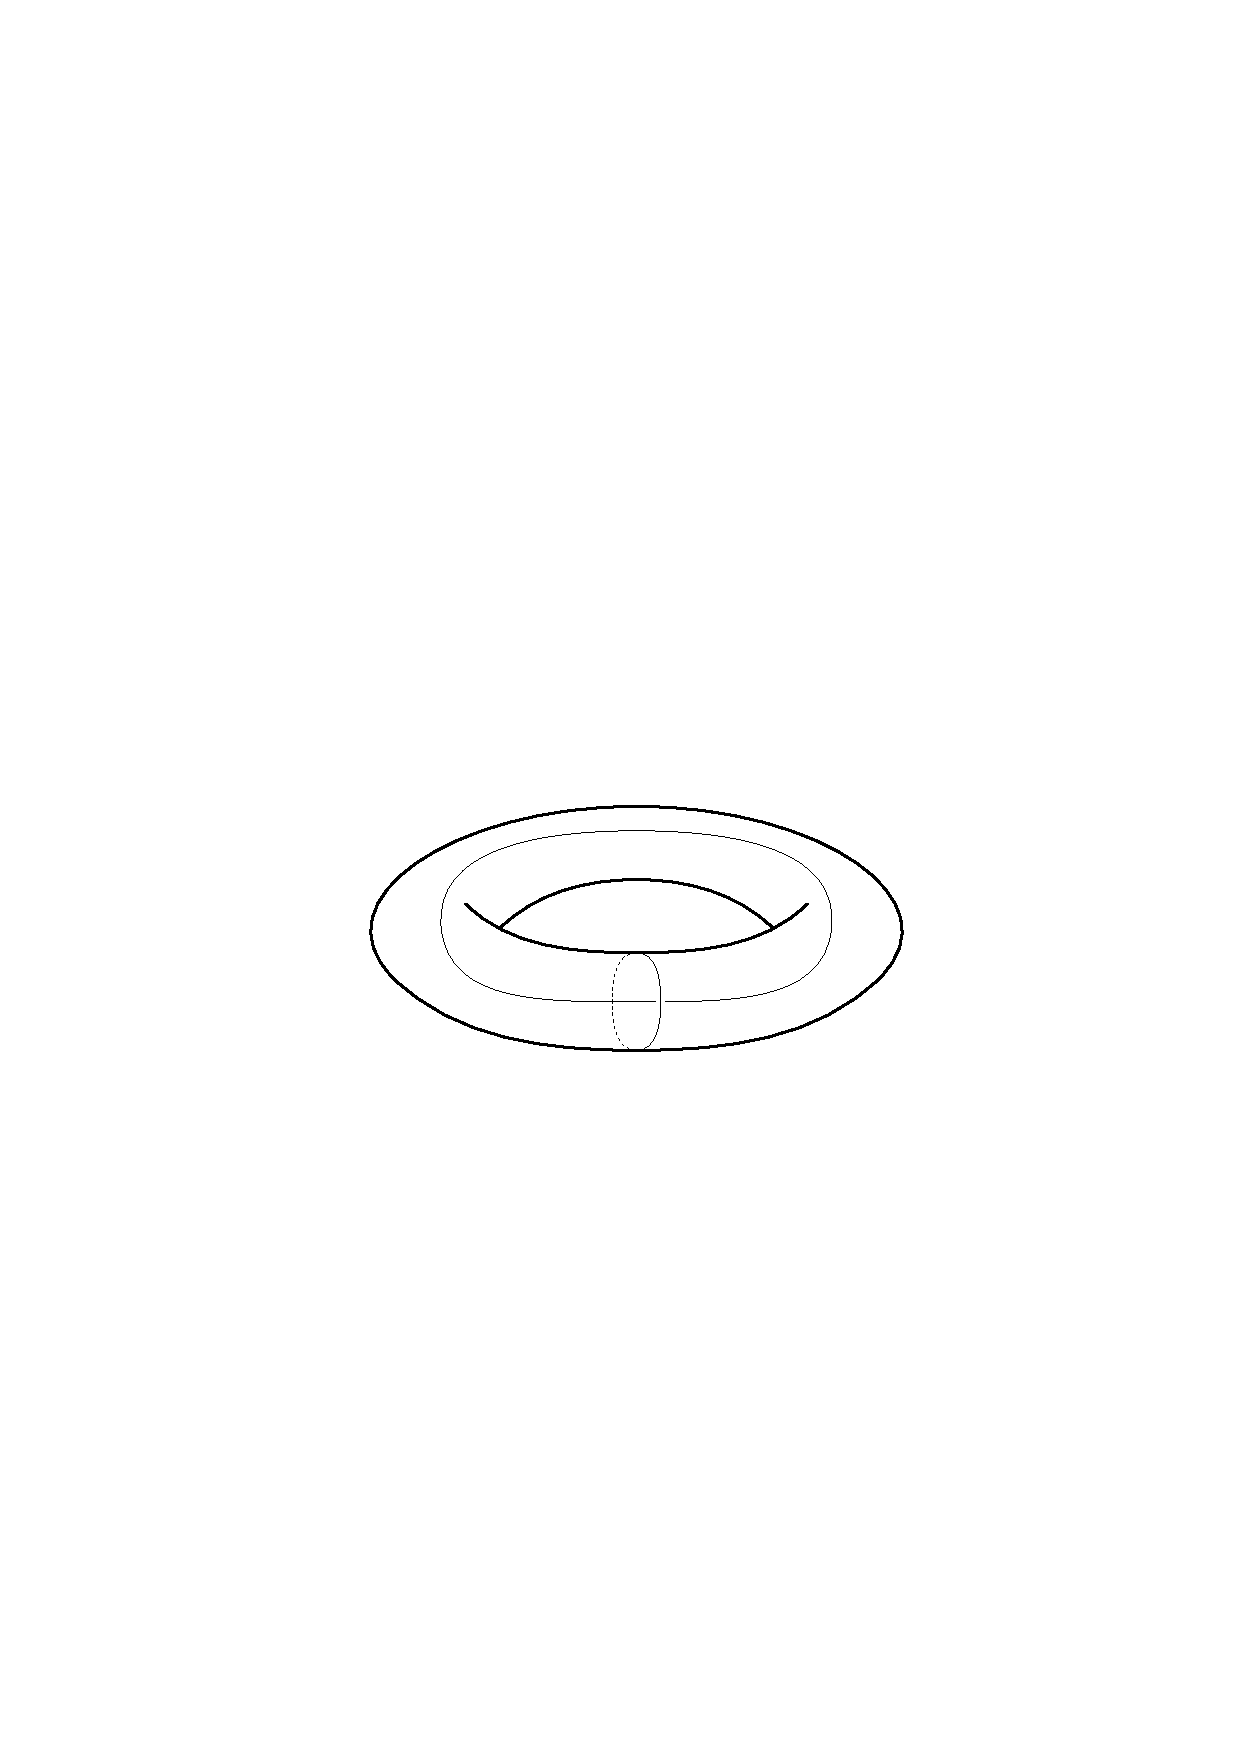
\includegraphics{chain_link_fence_knot_on_torus.pdf}
            }
            \caption{Chain Link Fence Knot on a Torus}
            \label{fig:chain_link_fence_knot_on_torus}
        \end{figure}
        \par\hfill\par
        This last definition borrows the same difficulty from graph theory.
        While attaching handles at all of the $g$ virtual crossings yields an
        embedding into $M\times\mathbb{R}$ where $M$ is the compact orientable
        surface of genus $g$, it may have been possible to use fewer handles.
        Consider again Figs.~\ref{fig:graph_has_genus_001} and
        \ref{fig:graph_has_genus_002} where we created an embedding into the
        genus 3 compact surface. The starting graph was actually planar and
        needs no additional handles (Fig.~\ref{fig:graph_has_genus_003}).
        The computation of the genus for graphs is known to be
        \textbf{NP-Complete} \cite{GareyJohnsonGraphCrossingNumberNPComplete}.
        \par\hfill\par
        While it is possible to compute the minimal genus of a virtual knot,
        we will not need such an algorithm. Our later work will be motivated
        by a more classical problem which is related to this difficulty.
        If one is given an extended Gauss code (a \textit{virtual knot}),
        is it possible to determine if there is a (classical) knot diagram
        that realizes this code? We can indeed do this in linear time.
        \par\hfill\par
        A valid Gauss code with $2N$ entries describes a virtual knot with
        $N$ crossings. Suppose we have embedded our virtual knot into
        $M\times\mathbb{R}$ where $M$ is a compact orientable surface of
        minimal genus such that projecting down the $\mathbb{R}$ component
        yields a knot diagram on $M$ with the desired extended Gauss code.
        We thus obtain a graph embedded into $M$ where the crossings form the
        vertices. The graph is 4-valent so by the hand-shaking theorem there
        are $2N$ edges. We are in effect decomposing $M$ into a CW complex with
        $N$ 0-cells, $2N$ 1-cells, and $F$ 2-cells. If we can compute $F$ we
        will obtain $g$ via Euler's formula:
        \begin{equation}
            V-E+F=2-2g
        \end{equation}
        Substituting $V=N$ and $E=2N$ we have:
        \begin{equation}
            g=\frac{2+N-F}{2}
        \end{equation}
        Hence computing $F$ yields $g$, and if $g\ne{0}$ we will know the
        extended Gauss code does not describe the knot diagram of a
        classical knot. We now show how to compute $F$.
        \par\hfill\par
        \begin{figure}
            \centering
            \includegraphics{thickened_crossings.pdf}
            \caption{Signed Thickened Crossings}
            \label{fig:thickened_crossings_chapt1}
        \end{figure}
        Thicken the knot projection so that the crossings look like
        Fig.~\ref{fig:thickened_crossings_chapt1}.
        Begin traveling along the thickened
        knot, following the orientation given by the Gauss code, and place your
        finger on the left wall at all times. When you come to a crossing,
        turn left so that your finger remains continuously on the wall of the
        thickened knot. Continue doing this until you return to your starting
        point. You will have just traced out an $n$-gon for some
        $n\in\mathbb{N}$. Attach a 2-cell by gluing along this polygon.
        Continue doing this until all $4N$ of the corners of the $N$ thickened
        crossings (again, see Fig.~\ref{fig:thickened_crossings_chapt1}) have
        been traveled. The total number of faces, which is the total number of
        cycles you've traveled, has now been computed. We require $4N$ steps,
        and so our algorithm does indeed run in linear time.
        \par\hfill\par
        The steps described translate to jumping between the entries in the
        Gauss code in a well-defined manner. \textit{Going left} means changing
        crossing type and then walking with or against the orientation.
        That is, if you come to entry \texttt{Ons}, with \texttt{n} the index
        and \texttt{s} the sign, jump ahead to \texttt{Uns}, changing crossing
        type. You then proceed to either the next entry in the Gauss code or
        the previous entry depending on the value of the sign \texttt{s}.
        This amounts to walking forwards or backwards. The correct direction
        can be computed from Fig.~\ref{fig:thickened_crossings_chapt1}.
        If you are at the final entry and need to proceed forward,
        loop back around to the
        start. Similarly, if you are at the starting entry and need to move
        backwards, jump ahead to the end of the Gauss code. By repeatedly
        doing this we can compute the number of cycles and consequently
        calculate the genus.
        \par\hfill\par
        Applying this algorithm to the standard 3-crossing trefoil (either the
        left handed or right handed) will yield 5 faces, giving us a genus of
        0. The chain link fence knot \texttt{O0+ U1+ U0+ O1+} produces 2 faces,
        and so we end up with a genus 1 knot diagram which can be embedded on
        the torus. The faces, and the reason for the name
        \textit{chain link fence}, can be easily seen if we conduct our drawings
        on the flat torus (Fig.~\ref{fig:chain_link_fence_knot_on_flat_torus}).
        If we lift to the universal cover of the torus, which is the Euclidean
        plane, we can see the two aforementioned faces, as well as a chain
        link fence pattern
        (Fig.~\ref{fig:chain_link_fence_knot_on_flat_torus_universal_cover}).
        \begin{figure}
            \centering
            \includegraphics{chain_link_fence_knot_on_flat_torus.pdf}
            \caption{Chain Link Fence Virtual Knot on a Flat Torus}
            \label{fig:chain_link_fence_knot_on_flat_torus}
        \end{figure}
        \begin{figure}
            \centering
            \resizebox{\textwidth}{!}{%
                \includegraphics{%
                    chain_link_fence_knot_on_flat_torus_universal_cover.pdf
                }
            }
            \caption{Lift of the Chain Link Fence to the Universal Cover}
            \label{fig:chain_link_fence_knot_on_flat_torus_universal_cover}
        \end{figure}
        \par\hfill\par
        It should be considered a pleasant bonus if a property of knots exists
        also for virtual knots. It is especially enjoyable when an
        algorithm can be copied for virtual knots with little or no additional
        effort. But, before proceeding, two warnings are worth mentioning.
        \par\hfill\par
        The operations of the Reidemeister moves are stricter for virtual knots
        via extended Gauss code. For classical knots, should we find
        \texttt{On Om} followed by \texttt{Un Um}, or any re-ordering thereof,
        we can apply Type II and delete the four entries from the code. This is
        not so for virtual knots. Indeed, were it true the chain link fence
        would be equivalent to the unknot. The sign is crucial for a correct
        description of Type II moves in the virtual setting. For a true
        Type II move the signs alternate. This in agreement with the fact that
        Type II does not change the writhe of a diagram. So, should we find
        \texttt{On+ Om-} followed by \texttt{Un+ Um-}, or any re-ordering
        thereof, we may apply Type II and delete the four entries, be it a
        classical or virtual knot.
        \par\hfill\par
        Lastly, the algorithm described previously computed the genus of a
        virtual knot \textit{diagram}, and not the minimal genus of all
        possible equivalent diagrams. By application of Type II it is possible
        to give the right-handed trefoil a genus 1 knot diagram, for example
        \texttt{O0+ U1+ O2+ O3- O4+ U0+ U3- U2+ O1+ U4+}. The Reidemeister
        moves may change the genus of a diagram.
    \section{Tait Graphs}
        The last representation we wish to describe is one of the original
        ones: the \textbf{Tait graph}. Like the braid group it will play a
        small role for us, but it is computationally useful and will lend
        us aid in devising algorithms later on. Projecting a knot or link down
        to a diagram yields a 4-valent graph where the crossings form the
        vertices. Being 4-valent with $N$ vertices (for the $N$ crossings),
        there will be $2N$ edges. Euler's formula states:
        \begin{equation}
            V-E+F=2
        \end{equation}
        \begin{figure}
            \centering
            \resizebox{0.5\textwidth}{!}{%
                \includegraphics{tait_graph_sign.pdf}
            }
            \caption{Signing for the Tait Graph}
            \label{fig:tait_graph_signs}
        \end{figure}
        Solving for $F$ tells us there are $N+2$ faces (including the unbounded
        face). Pick any face and place a dot in it.
        For every face adjacent to this by going \textit{directly across} a
        crossing (no going left, no going right) place another vertex and
        draw an edge to your original point. Moreover, color the edge blue or
        red depending on Fig.~\ref{fig:tait_graph_signs}
        (blue for positive, red for
        negative). Continue doing this recursively until all possible faces
        have been dotted and corresponding edges drawn. From planarity of the
        $N+2$ faces you will have placed dots in roughly half of them and a
        checkerboard pattern will appear. The resulting graph is one of the
        two possible Tait graphs for your diagram. The Hopf link is shown in
        Fig.~\ref{fig:hopf_link_tait_graph_002}.
        \begin{figure}
            \centering
            \resizebox{0.5\textwidth}{!}{%
                \includegraphics{hopf_link_tait_graph_002.pdf}
            }
            \caption{Tait Graph of the Hopf Link}
            \label{fig:hopf_link_tait_graph_002}
        \end{figure}
        \par\hfill\par
        Had you chosen a different face you may end up with the exact same
        graph, or the \textit{dual} graph in the plane. For example, using the
        standard right-handed trefoil diagram, choosing the face containing
        infinity will yield a \textit{trigon}, a 3-valent multigraph on two
        points, like in Fig.~\ref{fig:tait_graph_trefoil_001}. Had you chosen
        the inner most face you would have constructed the same graph. Choosing
        one of the clover like faces results in a cyclic graph, a triangle with
        colored edges as in Fig.~\ref{fig:tait_graph_trefoil_002}. The
        connection between these two is that they are duals in the plane.
        Note that the number of edges is the same, but the colorings are
        different. This can be realized by observing
        Fig.~\ref{fig:tait_graph_signs} and noting that the dual operation
        swaps the two pictures.
        \begin{figure}
            \centering
            \begin{minipage}[b]{0.49\textwidth}
                \centering
                \resizebox{0.8\textwidth}{!}{%
                    \includegraphics{tait_graph_trefoil_001}
                }
                \vspace{2em}
                \caption{Trefoil Tait Graph}
                \label{fig:tait_graph_trefoil_001}
            \end{minipage}
            \hfill
            \begin{minipage}[b]{0.49\textwidth}
                \centering
                \resizebox{0.8\textwidth}{!}{%
                    \includegraphics{tait_graph_trefoil_002}
                }
                \caption{Dual Trefoil Tait Graph}
                \label{fig:tait_graph_trefoil_002}
            \end{minipage}
        \end{figure}
        \par\hfill\par
        Tait graphs for equivalent knot diagrams should be equivalent,
        in some sense, and thus
        we need a mode of translating Reidemeister moves on knot diagrams to
        Reidemeister moves on Tait graphs. Fortunately this is quite visual and
        relatively easy to describe.
        \par\hfill\par
        Type I tells us we may remove loops in the knot diagram.
        A loop in the Tait graph
        corresponds to a \textit{leaf}, a vertex connected to a single other
        vertex, or a \text{loop}, an edge connecting a vertex to itself. Alas,
        should we find a loop in the graph we may delete it, and should there
        be a leaf we may delete both the vertex and the sole edge that falls
        upon it. The resulting Tait graph will be the Tait graph of an
        equivalent knot diagram (Fig.~\ref{fig:tait_graph_reidemeister_1}).
        \begin{figure}
            \centering
            \resizebox{0.5\textwidth}{!}{%
                \includegraphics{tait_graph_reidemeister_1.pdf}
            }
            \caption{Type I on Tait Graphs}
            \label{fig:tait_graph_reidemeister_1}
        \end{figure}
        \par\hfill\par
        Type II is almost as easy to describe. A Type II move tells us there
        will be a vertex of degree 2 (two edges connected to it) of different
        signs. Label the vertices $A$, $B$, and $C$, $B$ being the vertex in
        the center of degree 2. By pulling the under strand beneath the upper
        strand we are deleting one face and fusing two together
        (Fig.~\ref{fig:tait_graph_reidemeister_2_001}). This translates to
        deleting vertex $B$ and the two edges connected to it, but also
        combining vertices $A$ and $C$ into a single vertex with all
        corresponding edges connected to it.
        \par\hfill\par
        Had we chosen the dual graph of
        Fig.~\ref{fig:tait_graph_reidemeister_2_001} we would look for digonal
        subgraphs, or subgraphs with two vertices and two edges between them.
        Type II then says that should the signs of the two edges differ we
        can just delete them, but leave the vertices in place. To summarize,
        Type II amounts to deleting degree 2 vertices and the edges of digons
        whenever the edges alternate in sign.
        \begin{figure}
            \centering
            \includegraphics{tait_graph_reidemeister_2_001.pdf}
            \caption{Type II on Tait Graphs}
            \label{fig:tait_graph_reidemeister_2_001}
        \end{figure}
        \par\hfill\par
        Finally we come to Type III. While usually the most difficult to work
        with, the third Reidemeister move has the pleasant fact that the dual
        Tait graph yields an identical operation. So instead of two different
        kinds of Type III moves on Tait graphs, as we had with I and II,
        there is only one. Examining
        Fig.~\ref{fig:tait_graph_reidemeister_3_001} shows us how to conduct
        the operation, we perform the famous
        $\textrm{Y}-\Delta$ transform, a technique common in circuit theory
        and network analysis (see \cite{KennellyYDelta} for the original
        source material). That is, should we find a triangle in the Tait
        graph (with correct colorings for the edges) we may place a dot in the
        center of the triangle and redraw the edges to form a
        $\textrm{Y}$-shaped object. Similarly we may reverse this and transform
        a $\textrm{Y}$ into a triangle, or a $\Delta$.
        \par\hfill\par
        There is one more operation we may perform on Tait graphs that is not
        afforded to us in knot and link diagrams. At any point we may take the
        dual of the graph in the plane, being careful to draw the resulting
        edges with the proper colors. We may then perform the three
        Reidemeister moves on this new Tait graph, take the dual again, and
        so on. Demonstrating the equivalence of knots thus becomes a problem
        in showing two graphs are the same up to Reidemeister moves and planar
        duals.
        \begin{figure}
            \centering
            \includegraphics{tait_graph_reidemeister_3_001.pdf}
            \caption{Type III on Tait Graphs}
            \label{fig:tait_graph_reidemeister_3_001}
        \end{figure}
    \section{Modified Tait Graphs}
        Many of the assumptions in the description of the Tait graph used
        planarity of the knot diagram. Applying such a graph-theoretical
        idea to virtual knots will need modification. Indeed, the checkerboard
        pattern will be lost for some virtual knots since this is a
        phenomenon of the sphere. Consider the chain link fence knot on the
        flat torus (Fig.~\ref{fig:chain_link_fence_knot_on_flat_torus}).
        Regardless of which starting face you choose the other face will be
        given a dot as well. Rather than a checkerboard pattern of chosen
        faces on the torus we have instead covered the entire manifold. If we
        na\"{i}vely try to draw this we get
        Fig.~\ref{fig:chain_link_fence_knot_on_flat_torus_tait_graph_naive}. We
        see that the large face is connected to itself twice but the
        resuling edges are not loops that can be deleted by Type I moves.
        Rather, such loops  have information about the topology of the
        underlying manifold. Moreover, a graph is a set of vertices and a set
        of edges. The underlying manifold it is embedded on is immaterial.
        The graph in
        Fig.~\ref{fig:chain_link_fence_knot_on_flat_torus_tait_graph_naive}
        should thus be considered equivalent to
        Fig.~\ref{fig:chain_link_fence_knot_naive_tait_graph}. The issue with
        this is that
        Fig.~\ref{fig:chain_link_fence_knot_naive_tait_graph} is already the
        Tait graph of a (non-standard) Hopf link diagram.
        \begin{figure}
            \centering
            \begin{minipage}[b]{0.49\textwidth}
                \centering
                \resizebox{\textwidth}{!}{%
                    \includegraphics{%
                        chain_link_fence_knot_on_flat_torus_tait_graph_naive.pdf
                    }
                }
                \caption{Na\"{i}ve Virtual Tait Graph}
                \label{fig:chain_link_fence_knot_on_flat_torus_tait_graph_naive}
            \end{minipage}
            \hfill
            \begin{minipage}[b]{0.49\textwidth}
                \centering
                \resizebox{\textwidth}{!}{%
                    \includegraphics{%
                        chain_link_fence_knot_naive_tait_graph.pdf
                    }
                }
                \vspace{3em}
                \caption{Equivalent Graph}
                \label{fig:chain_link_fence_knot_naive_tait_graph}
            \end{minipage}
        \end{figure}
        \par\hfill\par
        The proposed work around is to have two types of edges (still positive
        and negative) as well as two types of vertices, which we'll call
        hollow and solid. At each of the crossings in the diagram place a
        hollow vertex. Choose a starting face and place a solid vertex in it.
        Draw an edge from the solid vertex to all hollow vertices that border
        the face, coloring the edges in accordance with
        Fig.~\ref{fig:tait_graph_signs}. For each face that can be reached
        by going across a crossing place another solid dot and connect the
        appropriate edges to hollow vertices. Continue doing this until all
        possible faces have been claimed. The result is our
        \textit{virtual} Tait graph. Fig.~\ref{fig:chain_link_fence_tait_graph}
        depicts this modification for the chain link fence.
        \begin{figure}
            \centering
            \includegraphics{chain_link_fence_tait_graph.pdf}
            \caption{Virtual Tait Graph}
            \label{fig:chain_link_fence_tait_graph}
        \end{figure}
        \par\hfill\par
        In the classical setting these new hollow vertices will all be
        degree 2, a fact derived from the checkerboard pattern that results.
        For non-classical knots the virtual Tait graph can become more
        complicated, but the hollow vertices will always be degree 2 or
        degree 4. This allows us to salvage the Reidemeister operations.
        \par\hfill\par
        For Type I we look for leaves where the leaf vertex is solid. We
        delete the solid vertex and the single hollow vertex adjacent to it,
        as well as all (2 or 4) edges falling on this hollow vertex. This
        results in merging the faces and removing the crossing. A similar
        operation can be done for loops, we look for a solid vertex with two
        edges connected to a hollow vertex. To ensure the loop
        corresponds to a Type I move we must insist that the hollow vertex be
        of degree 2. In this scenario we delete the two edges and the hollow
        vertex.
        \par\hfill\par
        The descriptions of Type II and Type III are similar to before, but
        planar duals must be replaced with duals on the appropriate manifold.
        This can be done pictorially by embedding the virtual knot diagram into
        the fundamental $4g$-gon for the genus $g$ surface the virtual knot
        lives in as we've done with the flat torus and the
        chain link fence knot. Later we will get some computational use out of
        this idea in our discussion of the Kauffman bracket.
    \section{Tait Graph Expansion}
        The next method of computation has two uses for us. Firstly, it is
        very efficient in terms of speed, and secondly it will give us an
        explicit formula for the Jones polynomial of \textbf{twist knots}.
        Later on we will appeal to this formula for calculations
        involving twist of over 90 crossings. The exponential nature of
        the algorithms we've thus far presented would otherwise prevent us
        from doing this.
        \par\hfill\par
        We start with the Tait graph. Given a knot or link diagram
        the smoothing operations for the Kauffman bracket can translate to
        operations on the Tait graph. This can be seen in
        Fig.~\ref{fig:tait_graph_kauffman_negative_smoothing} for negative
        (red) edges in the graph. For positive edges we would rotate the
        picture.
        \par\hfill\par
        \begin{figure}
            \centering
            \resizebox{0.5\textwidth}{!}{%
                \includegraphics{tait_graph_kauffman_negative_smoothing.pdf}
            }
            \caption{Smoothing a Negative Edge on the Tait Graph}
            \label{fig:tait_graph_kauffman_negative_smoothing}
        \end{figure}
        We see that the Kauffman relation tells us to contract and delete
        edges, which corresponds to merging and separating faces in the
        knot diagram. That is, if $T$ is the Tait graph of a knot diagram
        $K$, smoothing at the $n^{\small\textrm{th}}$ crossing corresponds
        to smoothing the $n^{\small\textrm{th}}$ edge via:
        \begin{align}
            \label{eqns:kauffman_tait_relation}
            \langle{T}\rangle
            &=\langle{{T^{n_{-}}_{\textrm{delete}}}}\rangle
            -q\langle{{T^{n_{-}}_{\textrm{contract}}}}\rangle\\
            \langle{T}\rangle
            &=\langle{{T^{n_{+}}_{\textrm{contract}}}}\rangle
            -q\langle{{T^{n_{+}}_{\textrm{delete}}}}\rangle
        \end{align}
        where $n_{\pm}$ indicates whether the edge is positive (blue) or
        negative (red), respectively.
        Separating disks will still result in disks, but
        merging is more subtle. If we are merging two distinct disks we are
        essentially creating a dogbone, which is still topologically a
        disk. The issue arises when the two dots in the left hand side of
        Fig.~\ref{fig:tait_graph_kauffman_negative_smoothing} represent
        the same face. In such an event we are creating a topological
        annulus, which is not allowed for Tait graphs since the vertices
        must represent disks in the knot diagram. The Kauffman reduction
        $\langle{\mathbb{S}^{1}\sqcup{K}}\rangle=(q+q^{-1})\langle{K}\rangle$
        comes to the rescue. The inner circle of our annulus corresponds to
        a cycle in the smoothing of the knot diagram. We may contract it to
        a point, turning our annulus into a disk, at the cost of a
        $q+q^{-1}$ term floating around.
        \begin{figure}
            \centering
            \resizebox{0.5\textwidth}{!}{%
                \includegraphics{tait_graph_reidemeister_1_dual.pdf}
            }
            \caption{Loops in the Tait Graph}
            \label{fig:tait_graph_reidemeister_1_dual}
        \end{figure}
        \par\hfill\par
        In the case of a blue edge we get:
        \begin{align}
            \langle{T}\rangle
            &=\langle{T^{n_{+}}_{\textrm{contract}}}\rangle
            -q\langle{T^{n_{+}}_{\textrm{delete}}}\rangle\\
            &=(q+q^{-1})\langle{T^{n_{+}}_{\textrm{delete}}}\rangle
            -q\langle{T^{n_{+}}_{\textrm{delete}}}\rangle\\
            &=q^{-1}\langle{T^{n_{+}}_{\textrm{delete}}}\rangle
        \end{align}
        For red we have:
        \begin{align}
            \label{eqn:tait_graph_kauffman_bracket_negative_loop_reduction}
            \langle{T}\rangle
            &=\langle{{T^{n_{-}}_{\textrm{delete}}}}\rangle
            -q\langle{{T^{n_{-}}_{\textrm{contract}}}}\rangle\\
            &=\langle{{T^{n_{-}}_{\textrm{delete}}}}\rangle
            -q(q+q^{-1})\langle{{T^{n_{-}}_{\textrm{delete}}}}\rangle\\
            &=-q^{2}\langle{{T^{n_{-}}_{\textrm{delete}}}}\rangle
        \end{align}
        This computation merely amounts to the fact that the Kauffman
        bracket polynomial is not invariant under Type I moves. It does,
        however, show the exact effect of Type I moves on a diagram, which
        is scaling by $-q^{2}$ or $q^{-1}$, depending on the sign of the
        introduced crossing.
        \par\hfill\par
        At the end of this deletion and contraction algorithm one will have
        dots on the plane. These corresponds to isolated faces bounded
        by cycles. To complete the computation we remove all of these
        points and replace them with $(q+q^{-1})^{m}$ where $m$ is the
        number of dots.
        \par\hfill\par
        As noted there are a lot of practical uses for this idea. Firstly
        it presents another algorithm, but one that operates on graphs.
        Second, and perhaps most important for us, it gives us a fairly
        simple means of computing the Jones polynomial of twist knots.
        Lastly, and perhaps most important for knot theorists, it can be
        modified and used to prove some of the original Tait conjectures.
        In \cite{ThistlethwaiteSpanningTree} the Kauffman bracket is
        computed by attaching monomials to each of the spanning trees of
        the Tait graph and then summing over them. This is a great
        theoretical tool, but also a powerful computational one.
        It is known that planar graphs have at most
        $O(r^{M})$ spanning trees with $r\approx{5.3}$ and where $M$ is the
        number of vertices \cite{NumberOfSpanningTrees}. This is the
        worst-case analysis, however, and luck occasionally strikes and
        gives us a much better bound. The Tait graph for the standard
        right and left trefoil diagrams have three spannings trees. Indeed,
        for $T_{2,\,p}$ torus knots there are $p$ spanning trees, reducing
        the computation to linear.
        \par\hfill\par
        We now put Eqns.~\ref{eqns:kauffman_tait_relation} to good use
        and compute the Jones polynomial of all twist knots. To do this
        we first describe twist knots. The twist knot with $n\in\mathbb{Z}$
        twists starts by performing $n$ Type I moves on the unit circle,
        creating a \textit{positive} Type I loop for $n>0$ and a
        \textit{negative} Type I loop for $n<0$. To create a non-trivial
        knot we then stretch the ends around and link them together by
        cutting at a point, lacing, and then tying
        (see Fig.~\ref{fig:twist_knot_001}).
        \begin{figure}
            \centering
            \resizebox{0.6\textwidth}{!}{%
                \includegraphics{twist_knot_001.pdf}
            }
            \caption{Twist Knots}
            \label{fig:twist_knot_001}
        \end{figure}
        \begin{figure}
            \centering
            \resizebox{0.6\textwidth}{!}{%
                \includegraphics{twist_knot_tait_graph_001.pdf}
            }
            \caption{Tait Graph of Twist Knots}
            \label{fig:twist_knot_tait_graph_001}
        \end{figure}
        By choosing one of the inner loop faces as the start we obtain a
        pleasant Tait graph to work with
        (Fig.~\ref{fig:twist_knot_tait_graph_001}). By performing the
        Kauffman relation on the bottom right-most edge we obtain
        Fig.~\ref{fig:twist_knot_tait_graph_kauffman_relation}. The
        1-smoothing yields a digon with a chain attached ending in a leaf.
        Noting that the dual of a positive leaf results in a negative loop,
        we may use
        Eqn.~\ref{eqn:tait_graph_kauffman_bracket_negative_loop_reduction} to
        see that deleting a positive leaf scales the Kauffman bracket by
        $-q^{2}$. For the $K_{N}$ twist knot there will be
        $N-1$ vertices along the chain, deleting all of them yields
        $(-q^{2})^{N-1}\langle{H}\rangle$ where $H$ is the knot diagram
        corresponding to the digon, which happens to be the Hopf link.
        \par\hfill\par
        The 0-smoothing is even nicer, we have obtained the Tait graph for
        the $K_{N-1}$ twist knot. We thus have the following recursion
        relation.
        \begin{figure}
            \centering
            \includegraphics{twist_knot_tait_graph_kauffman_relation.pdf}
            \caption{Kauffman Relation for the Tait Graph of Twist Knots}
            \label{fig:twist_knot_tait_graph_kauffman_relation}
        \end{figure}
        \begin{align}
            \langle{K_{N+1}}\rangle
            &=\langle{K_{N}}\rangle
            -q(-q^{2})^{N}\langle{H}\rangle\\
            &=\langle{K_{N}}\rangle
            +(-1)^{N+1}q^{2N+1}\langle{H}\rangle
        \end{align}
        We may expand this recusion out $N$ times until we get $K_{1}$,
        which is the left-handed trefoil. Our formula becomes
        \begin{equation}
            \langle{K_{N+1}}\rangle
            =\langle{K_{1}}\rangle
            +\langle{H}\rangle
            \sum_{k=1}^{k}(-1)^{k+1}q^{2k+1}
        \end{equation}
        Using the geometric series we get
        \begin{equation}
            \langle{K_{N+1}}\rangle
            =\langle{K_{1}}\rangle+\langle{H}\rangle
            \frac{q^{3}}{1+q^{2}}\big(1+(-1)^{N+1}q^{2N}\big)
        \end{equation}
        so the computation of the Kauffman bracket for twist knots is
        reduced to the left-handed trefoil and the Hopf link (in their
        standard diagrams). The left-handed trefoil produces
        \begin{equation}
            \langle{K_{1}}\rangle=(q+q^{-1})(q^{-2}-1-q^{4})
        \end{equation}
        and the Hopf link yields
        \begin{equation}
            \langle{H}\rangle=
            (q+q^{-1})(q^{-1}+q^{3})
        \end{equation}
        After computing the writhes of the diagram and normalizing
        by $q+q^{-1}$ we obtain the Jones polynomial:
        \begin{equation}
            J_{K_{N}}(q)
            =\begin{cases}
                \frac{q^{6}+q^{2}-q^{6-2N}+q^{-2N}}{1+q^{2}}
                &N\textrm{ even}\\
                \frac{1+q^{-4}+q^{-2N}-q^{-2N-6}}{1+q^{2}}
                &N\textrm{ odd}
            \end{cases}
        \end{equation}
        This computation holds for $N>0$. For $N<0$ we use the
        reflection formula by noticing that $K_{N}$ and $K_{-1-N}$ are
        mirrors of each other. We could also repeat the Tait graph
        computation using red edges, either works.
        \par\hfill\par
        We can get an algorithm for virtual knots out of the Tait graph
        if we use the modifications presented in the first chapter. Given
        the virtual Tait graph for a virtual knot diagram, for any
        crossing (hollow vertex) there are three possibilities:
        \begin{enumerate}
            \item There are two red edges incident.
            \item There are two blue edges incident.
            \item There are two red edges and two blue edges incident.
        \end{enumerate}
        Smoothings in the knot diagram equate to deleting hollow vertices,
        and the Kauffman relations tell us how to get a polynomial out of this
        from the modified Tait graph. For the first two possibilities we
        have Eqns.~\ref{eqns:kauffman_tait_relation}. An algorithm for
        virtual knots will be obtained once we've figured out how to
        resolve a hollow vertex of degree 4. To do this we note that
        a 0-smoothing will cut the red edges and contract the blue ones,
        whereas a 1-smoothing does the opposite, cutting blue edges and
        contracting red ones. As before we must be careful in this
        contraction, should a loop be created we must remove it and then
        scale the polynomial by $-q^{2}$ or $q^{-1}$, depending on the
        color of the edge for the loop. And that's it, we can now compute
        the Kauffman bracket for virtual Tait graphs as well.
        \bibliographystyle{annotate}
        \bibliography{bib.bib}
\end{document}
